\chapter{Segmentación de imágenes con un solo umbral con funciones de Dombi}\label{monoumbral}

En este capítulo en primer lugar se presentarán todas las herramientas algorítmicas que se van a utilizar para llevar a cabo los experimentos de este trabajo, haciendo énfasis en la forma de utilización para funciones de Dombi. Seguidamente se mostarán los resultados obtenidos para la segmentación monoumbral con estas funciones.


\section{Métodos algorítmicos de segmentación de un único umbral}\label{sec:algoritmosmono}
\documentclass[main]{subfiles}

\begin{document}

% ALGORITMO 1 GENERAL
\subsection{Algoritmo general maximizando la similitud}

Este algoritmo, que se presenta en \cite{art:barrenechea}, pretende conseguir obtener un único umbral a partir de la maximización de la similitud.

\begin{algorithm}
\begin{algorithmic}[1]
\REQUIRE Una imagen $Q$ en escala de grises donde sus píxeles estén entre $0$ y $L-1$.
\ENSURE El umbral $t$ a partir del cual se divide $Q$ en objeto y fondo.
\FOR {$t$:=0 hasta $L-1$}
\STATE Divisón de la imagen en dos clases $C_b(t)$ y $C_o(t)$. Para cada una de estas clases, calcular su media: $m_b(t)$ y $m_o(t)$.
\STATE Construcción del conjunto difuso $Q_t$.
\STATE Calcular la $SM(\tilda1, Q_t)$. \label{lin:alg1:similitud}
\ENDFOR
\RETURN \{$t$ | max($SM$)\}
\end{algorithmic}
\caption{Maximización de la similitud}\label{alg:algoritmo1}
\end{algorithm}

En el algoritmo anterior se necesitan varias definiciones que se explican a continuación. En primer lugar, se describe el método de creación de los conjuntos difusos para lo que se explica previamente el cálculo de las medias para el fondo y el objeto.

\begin{definition}\label{def:mediasmonoumbral}
Teniendo en cuenta la definición de la media de una imagen que se ha dado en el apartado \ref{sec:notacion}, y disponiendo del histograma de la imagen $h(q)$ para un cierto nivel $q, \forall q\in Q$, se define la media de los píxeles del fondo como:
$$m_b(t)=\frac{\sum_{q=0}^{t}qh(q)}{\sum_{q=0}^{t}h(q)};$$
y para los píxeles del objeto como:
$$m_o(t)=\frac{\sum_{q=t+1}^{L-1}qh(q)}{\sum_{q=t+1}^{L-1}h(q)}.$$
\end{definition}

\begin{definition}\label{def:conjuntodifusomonoumbral}
Dada $Q$, una imagen en la escala de L niveles de gris, y $t$, un nivel de gris de forma que $0\leq t\leq L-1$. Teniendo en cuenta que $F$ es una función $REF$ ya que la $REF \circ \varphi$ lo es, se define el conjunto
$$Q_t = \{(q, \mu_{Q_t}(q)|q\in \{0,1,\dots, L-1\}\}$$
teniendo en cuenta que
$$\mu_{Q_t}(q) = \left\{ \begin{aligned}
    F \left(\frac{q}{L-1}, \frac{m_b(t)}{L-1} \right) = \varphi\left(REF\left(\frac{q}{L-1}, \frac{m_b(t)}{L-1} \right)\right) & \quad\text{si}\ q\leq t,\\
    F \left(\frac{q}{L-1}, \frac{m_o(t)}{L-1} \right) = \varphi\left(REF\left(\frac{q}{L-1}, \frac{m_o(t)}{L-1} \right)\right) & \quad\text{si}\ q> t.
 \end{aligned}\right.$$
 \end{definition}

\begin{remark}
Como parece lógico a la vista de la definición \ref{def:conjuntodifusomonoumbral}, es necesario poder enumerar aquellas funciones que se utilizarán como $REF$ y como automorfismo $\varphi$. Para todos los casos se tendrá $\varphi = x$ y, además, se distinguirán las siguientes funciones $REF$:
\begin{enumerate}
    \item $REF(x,y)=1-\abs{x-y}$
    \item $REF(x,y)=1-\abs{x-y}^2$
    \item $REF(x,y)=1-\abs{x-y}^{0.5}$
    \item $REF(x,y)=(1-\abs{x-y})^2$
    \item $REF(x,y)=(1-\abs{x-y})^{0.5}$
\end{enumerate}
\end{remark}

Debido a la formulación de este tarbajo, se sustituirá la aplicación anterior que actúa como función $F$ en la definición \ref{def:conjuntodifusomonoumbral} por la función de Dombi \cite{art:dombi} definidas en \ref{def:dombi}. De esta forma, en este caso, los conjuntos difusos quedarán como explica la ecuación \ref{eq:conjdifusosdombimono}.
\begin{equation} \label{eq:conjdifusosdombimono}
    \mu_{Q_t}(q) = \left\{ \begin{aligned}
        F \left(w,\left(\frac{q}{L-1}, \frac{m_b(t)}{L-1}\right)\right) = \frac{1}{2}\left(1 + \left(1-2\frac{q}{L-1}\right)^w\cdot\left(1-2\frac{m_b(t)}{L-1}\right)^w\right)& \quad\text{si}\ q\leq t,\\
        F \left(w,\left(\frac{q}{L-1}, \frac{m_o(t)}{L-1}\right)\right) = \frac{1}{2}\left(1 + \left(1-2\frac{q}{L-1}\right)^w\cdot\left(1-2\frac{m_o(t)}{L-1}\right)^w\right)& \quad\text{si}\ q> t.
     \end{aligned}\right.
\end{equation}
%\REV{Está bien definido cómo he metido el parámetro d??}
Además, el último paso del bucle, en la línea \ref{lin:alg1:similitud} (Algoritmo \ref{alg:algoritmo1}=, se lleva a cabo la busqueda de la similitud frente al conjunto $\tilda1$. Para poder llevar a cabo este cálculo, tal y como se especifica en la definición \ref{def:similitud}, necesitamos utilizar una función $REF$, que será $REF_2=1-\abs{x-y}^2$, y la agregación $M$, la media aritmética ($M=\frac{i=1}{n}\sum_1^n x_i$). De esta forma, quedará como sigue:
\begin{equation}\label{eq:similitud}
    SM(\tilda1, Q_{t}) = M^{L-1}_{q=0}(h(q)\cdot REF_2(1,\mu_{Q_t}(q)))
\end{equation}


% ALGORITMO DEL ÁREA
\subsection{Algoritmo del área}

Este algoritmo, que se presenta en \cite{art:barrenechea} también, pretende hayar un nuevo umbral a través de la creación de una función $REF$, tal y como se explica en el teorema \ref{prop:contruccionref}.

\begin{algorithm}
\begin{algorithmic}[1]
\REQUIRE Una imagen $Q$ en escala de grises donde sus píxeles estén entre $0$ y $L-1$.
\ENSURE El umbral $t$ a partir del cual se divide $Q$ en objeto y fondo.
\FOR {$t$:=0 hasta $L-1$}
\STATE \begin{equation*}\begin{split}
A(Q_t)= \sum_{q=0}^{t} h(q)\varphi_1^{-1}\left(1-\abs{\varphi_2\left(\frac{q}{L-1}\right)-\varphi_2\left(\frac{m_b(t)}{L-1}\right)}\right) + \\ \sum_{q=t+1}^{L-1} h(q)\varphi_1^{-1}\left(1-\abs{\varphi_2\left(\frac{q}{L-1}\right)-\varphi_2\left(\frac{m_o(t)}{L-1}\right)}\right)
\end{split}\end{equation*}
\ENDFOR
\RETURN \{$t$ | max($A(Q_t)$)\}
\end{algorithmic}
\caption{Umbralización del área}\label{alg:algoritmo2}
\end{algorithm}

Esta es, realmente, una nueva versión del algoritmo de maximización de similitud anterior. Por esta razón, se prepara una formulación para conocer la relación de la similitud en función del área ($A$) que se ha calculado. Se intentará, por tanto, simplificarlo retirando la función de similitud $SM$.
\begin{proposition}
Dada una agregación $M$, la media aritmética, y la función $REF_2$, una función de equivalencia restringida formada según la definición \ref{def:ref}. Si se construyen dos conjuntos difusos $Q_{t_1}$ y $Q_{t_2}$ de acuerdo a definición \ref{def:conjuntodifusomonoumbral} de la imagen $Q$. Si disponemos de una medida de similitud presentada en \ref{def:similitud} podemos afirmar que:
$$SM(\tilda1, Q_{t_1})\leq SM(\tilda1, Q_{t_1})\quad \text{si y sólo si}\quad A(Q_{t_1})\leq A(Q_{t_1})$$
\end{proposition}
\begin{proof}
Sabiendo que $REF(1,x)=x, \xinunitinterval$, entonces:
$$SM(\tilda1, Q_{t_1})
= \frac{1}{\sum_{q=0}^{L-1}h(q)}\sum_{q=0}^{L-1}\left( h(q)REF_2(1, \mu_{Q_{t_1}}(q))\right)
= \frac{1}{\sum_{q=0}^{L-1}h(q)}\sum_{q=0}^{L-1}\left( h(q)\mu_{Q_{t_1}}(q)\right)
= \frac{A(Q_{t_1})}{\sum_{q=0}^{L-1}h(q)}.$$
Por esta razón, también se podrá decir que $SM(\tilda1, Q_{t_2}) = \frac{A(Q_{t_2})}{\sum_{q=0}^{L-1}h(q)}$ lo que prueba la proposición anterior.
\end{proof}

En este algoritmo, se utilizan 3 pares de automorfismos para darle forma al área.

%\begin{table}[h!]\begin{center}
%\resizebox*{14cm}{!}{\begin{tabular}{c||c|c||c}
%&$\varphi_1$ & $\varphi_2$ & $A(Q_t)$\\\hline\hline
%(1)&$x$ & $x$ & $\sum_{q=0}^{L-1} h(q) - \left(\sum_{q=0}^{t} \left(1-\abs{\frac{q}{L-1}-\frac{m_b(t)}{L-1}}\right) - \sum_{q=t+1}^{L-1} \left(1-\abs{\frac{q}{L-1}-\frac{m_o(t)}{L-1}}\right)\right)$ \\\hline
%(2)&$x^d$ & $x$ & $\sum_{q=0}^{t} h(q) \left(1-\abs{\frac{q}{L-1}-\frac{m_b(t)}{L-1}}\right) - \sum_{q=t+1}^{L-1} h(q) \left(1-\abs{(\frac{q}{L-1}-\frac{m_o(t)}{L-1}}\right)$ \\\hline

%(3)&$x^1-(1-x)^{1/2}$ & $x$ & $\sum_{q=0}^{L-1} h(q) - \left(\sum_{q=0}^{L-1} h(q) \left(\frac{q}{L-1}-\frac{m_b(t)}{L-1}\right)^2 - \sum_{q=t+1}^{L-1} h(q) \left(\frac{q}{L-1}-\frac{m_o(t)}{L-1}\right)^2\right)$ \\\hline

%\end{tabular}}\end{center}
%\caption{Porcentajes de acierto para los diferentes \datasets y configuraciones para {\em train}.\label{resultTrain}}
%\end{table}

\begin{enumerate}\label{enum:funcionesalg2}
    \item Se toma $\varphi_1(x) = \varphi_2(x) = x, \xinunitinterval$.
    $$A(Q_t) = sum_{q=0}^{L-1} h(q) - \left(\sum_{q=0}^{t} \left(1-\abs{\frac{q}{L-1}-\frac{m_b(t)}{L-1}}\right) - \sum_{q=t+1}^{L-1} \left(1-\abs{\frac{q}{L-1}-\frac{m_o(t)}{L-1}}\right)\right)$$
    \item Se toma $\varphi_1(x) = x^d \text{ con } d\neq0, \xinunitinterval \text{ y } \varphi_2(x)=x, \xinunitinterval$.
    $$\sum_{q=0}^{t} h(q) \left(1-\abs{\frac{q}{L-1}-\frac{m_b(t)}{L-1}}\right) - \sum_{q=t+1}^{L-1} h(q) \left(1-\abs{\frac{q}{L-1}-\frac{m_o(t)}{L-1}}\right)$$
    \item Se toma $\varphi_1(x) = 1-\sqrt{1-x}, \xinunitinterval \text{ y } \varphi_2(x)=x,\xinunitinterval$
    $$\sum_{q=0}^{L-1} h(q) - \left(\sum_{q=0}^{L-1} h(q) \left(\frac{q}{L-1}-\frac{m_b(t)}{L-1}\right)^2 - \sum_{q=t+1}^{L-1} h(q) \left(\frac{q}{L-1}-\frac{m_o(t)}{L-1}\right)^2\right)$$
\end{enumerate}
En total, se dispondrá de 4 versiones diferentes. Se debe tener en cuenta que en la en el par (2) de automorfismos se dispondrá de $d=0,5$ y $d=2$.

% ALGORITMO 3
\subsection{Algoritmo de selección del umbral óptimo}\label{sec:algoritmo3}

\begin{definition}\label{def:conjuntoHmonoumbral}
Dada $Q$, una imagen en la escala de L niveles de gris, y $t$, un nivel de gris de forma que $0\leq t\leq L-1$, se calcula su conjunto $H(Q_t)$ como
$$H(Q_t) = \{(q, \mu_{H(Q_t)}(q)|q\in \{0,1,\dots, L-1\}\}$$
teniendo en cuenta que
$$\mu_{Q_t}(q) = \left\{ \begin{aligned}
    \frac{m_b(t)}{L-1} & \quad\text{si}\ q\leq t,\\
    \frac{m_o(t)}{L-1} & \quad\text{si}\ q> t.
 \end{aligned}\right.$$
 \end{definition}

En el algoritmo, necesitaremos, después, calcular la similitud que existe entre el conjunto $Q_t$ y el conjunto $H(Q_t)$. Para ello aplicamos la definición \ref{def:similitud}:
$$SM(Q_t, H(Q_t)) = M^{L-1}_{q=0}(h(q)REF(\mu_{Q_t}(q), \mu_{H(Q_t)}(q)))$$
Tendremos en cuenta que $M$ seguirá siendo la media aritmética y $REF=1-\abs{x-y}^2 \xinunitinterval$. Si a través de la uniformidad simplificamos la expresión anterior, obtendremos:
$$SM(Q_t, H(Q_t)) = \frac{1}{\sum_{q=0}^{L-1}h(q)} \sum_{q=0}^{L-1}\left(h(q)(1-(\mu_{Q_t}(q)-\mu_H{(Q_t)}(q))^2)\right)$$

\begin{algorithm}[!ht]
\begin{algorithmic}[1]
\REQUIRE Una imagen $Q$ en escala de grises donde sus píxeles estén entre $0$ y $L-1$.
\ENSURE El umbral óptimo $t^*$ a partir del cual se divide $Q$ en objeto y fondo.
\FOR {$t$:=0 hasta $L-1$}
\STATE Calcular los conjuntos $Q_t$ como se describe en la definición \ref{def:conjuntodifusomonoumbral}.
\STATE Calcular los conjuntos $H$ como se muestra en la definición \ref{def:conjuntoHmonoumbral}.
\STATE Calcular la $SM(Q_t, H(Q_t))$.
\ENDFOR
\RETURN \{$t*$ | max($SM$)\}
\end{algorithmic}
\caption{Selección del umbral óptimo}\label{alg:algoritmo3}
\end{algorithm}



%ALGORITMO GLOBAL
\subsection{Otros algoritmos}\label{sec:otrosalgoritmos}
\subsubsection{Algoritmo de umbralización global}\label{sec:algoritmoglobal}

Entre los algoritmos que se encargan de segmentar la imagen con un único umbral, este es el más simple aunque en ocasiones podemos obtener resultados suficientemente buenos según que aplicación queramos darle.

\begin{algorithm}[!ht]
\begin{algorithmic}[1]
\REQUIRE Una imagen $Q$ en escala de grises donde sus píxeles estén entre $0$ y $L-1$.
\ENSURE El umbral óptimo $t$ a partir del cual se divide $Q$ en objeto y fondo.
\STATE $t = 128$;
\COMMENT{Se selecciona un umbral inicial cualquiera, aquí se tomará el valor medio de los posibles}
\REPEAT
\STATE $tant = t$;
\STATE $G1 = \{(x, y) | q(x, y) > t0\}$
\STATE $G2 = \{(x, y) | q(x, y) \leq t0\}$
\STATE $m1 = \frac{1}{\abs{G1}} \sum_{i\in G1} i$
\STATE $m2 = \frac{1}{\abs{G2}} \sum_{i\in G2} i$
\STATE $t = \frac{m1+m2}{2}$
\UNTIL {$\abs{tant-t} < \varepsilon$}
\COMMENT {El valor $\varepsilon$ es un cierto error dispuesto por el programador.}
\RETURN $t$
\end{algorithmic}
\caption{Umbralización global.}\label{alg:global}
\end{algorithm}

En este sentido, para el buen funcionamiento del algoritmo es necesario que la imagen tenga una clara separación entre el objeto y el fondo, expresada con un valle en el histograma de la imagen. Se debe tener cuidado al elegir el parámetro $\varepsilon$ ya que de él depende el número de iteraciones del bucle. Normalmente, conforme este crece, menor es el número de iteraciones necesarias para un resultado adecuado.


% ALGORTIMO DE OTSU
\subsubsection{Algoritmo de Otsu}\label{sec:algoritmootsu}

El algoritmo de Otsu \cite{art:otsu} basa su técnica de umbralización, también, en el histograma de la imagen que recibe. Para ello, trata las probabilidades que se le ortorgan a cada uno de los niveles de gris de los que dispone la imagen. Si tomamos una imagen $Q$ que tenga sus intensidades entre $[1, 2, \dots, L]$, podremos expresar la probablidad de cada intensidad como
$$p_i = \frac{n_i}{N}, \quad p_i \geq 0\quad\text{ sabiendo que }\quad\sum_{i=0}^{L-1}p_i=1$$
siendo $n_i$ el número de píxeles de intensidad $i$ y $N$ el número total de píxeles en la imagen $Q$.

Ahora, supondremos que podemos clasificar los elementos de la imagen en dos clases, $C_0$ y $C_1$ que tendrán a los píxeles $[0,\dots,k]$ y $[k+1,\dots,L-1]$ respectivamente. Definirán su probabilidad como
$$\omega_0 = \Pr(C_0) = \sum_{i=0}^{t}p_i=\omega_0(t)\qquad\text{y}\qquad
\omega_1 = \Pr(C_1) = \sum_{i=t+1}^{L-1}p_i=\omega_1(t)$$
y su media como
$$\mu_0=\sum_{i=0}^t i \Pr(i|C_0) = \sum_{i=0}^t \frac{ip_i}{\omega_0} = \frac{\mu(t)}{\omega(t)}\qquad\text{y}\qquad
\mu_1=\sum_{i=t+1}^{L-1} i \Pr(i|C_1) = \sum_{i=t+1}^{L-1} \frac{ip_i}{\omega_1} = \frac{\mu_T-\mu(t)}{1-\omega(t)}$$
donde
$$\omega(k)\sum_{i=0}^k ip_i   \qquad\text{y}\qquad   \mu(k)=\sum_{i=0}^k ip_i$$

Por último, se puede definir
$$\mu_T = \mu(L-1) = \sum_{i=0}^{L-1} ip_i$$
y todas estas definiciones podemos asegurar que cumplirán que
$$\omega_0\mu_0+\omega_1\mu_1 = \mu_T   \qquad\text{y}\qquad   \omega_0+\omega_1 = 1$$
Con la intención de evaluar lo adecuado o no que es cada umbral $t$, podemos definir la varianza de cada uno como
$$\sigma_B^2(t) = \omega_0(\mu_0-\mu_T)^2 + \omega_1(\mu_1-\mu_T)^2 = \omega_0\omega_1(\mu_1-\mu_0)^2$$
Con todo ello, para encontrar el umbral óptimo $t^*$ sólo deberemos encontrar aquella varianza que maximice a las demás.
$$\sigma_B^2(t^*) = \max_{1\leq k <L}\left\{\sigma_B^2(t)\right\}$$

Al resumir todo lo anterior en lenguaje algorítmico se encuentra:
%\REV{El umbral de 1..L en vez de 0..L-1} Solucionado, se queda igual que todos de 0..L

\begin{algorithm}
\begin{algorithmic}[1]
\REQUIRE Una imagen $Q$ en escala de grises donde sus píxeles estén entre $0$ y $L-1$.
\ENSURE El umbral óptimo $t^*$ a partir del cual se divide $Q$ en objeto y fondo.
\FOR {$t$:=0 hasta $L-1$}
\STATE $\omega_0$(t) = $\sum_{i=1}^{t}p_i$
\STATE $\mu_0$(t) = $\sum_{i=1}^t \frac{ip_i}{\omega_0}$
\STATE $\omega_1$(t) = $\sum_{i=t+1}^{L}p_i$
\STATE $\mu_1$(t) = $\sum_{i=t+1}^L \frac{ip_i}{\omega_1}$
\STATE $\sigma_B^2(t) = \omega_0\omega_1(\mu_1-\mu_0)^2$
\ENDFOR
\RETURN \{$t^*$ | $max_t(\sigma_B^2$)\}
\end{algorithmic}
\caption{Selección del umbral óptimo según Otsu.}\label{alg:otsu}
\end{algorithm}


% ALGORITMO DE LA ENTROPÍA DE RENYI
\subsubsection{Algoritmo de maximización de la entropía de Renyi}\label{sec:algoritmorenyi}
Este algoritmo, enunciado en \cite{art:sahoo}, busca el umbral óptimo de la imagen a través de la maximización de la entropía que se produce en la imagen definida por Renyi. Al igual que en el algoritmo de Otsu se empieza definiendo dos clases, la correspondiente al fondo y la del objeto. Para cada una de ellas se define su probabilidad
$$p(C_0)=\sum_{i=0}^{t}p_i\qquad\text{y}\qquad p(C_1)=\sum_{i=t+1}^{L-1}p_i$$
donde con ambas probabilidades se cumple que $p(C_0)+p(C_1)=1$.

%Método de el anterior KAPUT
%$$H_T=-\sum_{i=0}^{L-1} p_i \ln p_i$$
%$$H_{C_0}(t)=-\sum_{i=0}^{t} \frac{p_i}{p(C_0)} \ln \frac{p_i}{p(C_0)}$$
%$$H_{C_1}(t)=-\sum_{i=t+1}^{L-1} \frac{p_i}{p(C_1)} \ln \frac{p_i}{p(C_1)}$$
%$$p(C_0)\sum_{i=0}^{t}p_i$$
%$$p(C_1)\sum_{i=0}^{t}p_i$$
%$$p(C_0)+p(C_1)=1$$

%$$C_0:\frac{p_0}{p(C_0)},\frac{p_1}{p(C_0)},\dots,\frac{p_t}{p(C_0)}$$
%$$C_1:\frac{p_0}{p(C_1)},\frac{p_1}{p(C_1)},\dots,\frac{p_t}{p(C_1)}$$
%$$H_{T}^{\alpha}(t) = \frac{1}{1-\alpha}\ln \sum_{i=0}^{L-1}\left(p_i\right)^\alpha \quad\text{con }\alpha\neq 1$$
A continuación se define la entropía para ambas clases sabiendo que $\alpha\neq 1$.
$$H_{C_0}^{\alpha}(t) = \frac{1}{1-\alpha}\ln \sum_{i=0}^{t}\left(\frac{p_i}{p(C_0)}\right)^\alpha \qquad\text{y}\qquad
H_{C_1}^{\alpha}(t) = \frac{1}{1-\alpha}\ln \sum_{i=t}^{L-1}\left(\frac{p_i}{p(C_1)}\right)^\alpha$$

Llegado este punto, se puede encontrar el umbral óptimo $t^*(\alpha)$ aquel que maximice la suma de las entropías de las clases:
$$t^*(\alpha)=\max_{0\leq t<L}\left\{H_{C_0}^{\alpha}(t)+H_{C_1}^{\alpha}(t)\right\}.$$

Por medio de experimentación se ha comprobado que el umbral anterior no es igual para todos los valores de $\alpha$. Este hecho se formaliza de la siguiente forma:
$$t^*(\alpha)=\left\{\begin{aligned}
    t^*_1 & \text{  si  }0<\alpha<1,\\
    t^*_2 & \text{  si  }\alpha\rightarrow1,\\
    t^*_3 & \text{  si  }1<\alpha<\infty.
\end{aligned}\right.$$

Por esta razón, se hace necesario emcontrar un umbral $t$ que no sea dependiente de $\alpha$. Para ello se deben calcular un umbral para cada una de las 3 situaciones enumeradas y ordenarlos de mayor a menor, algo que simbolizaremos como $\tonee\leq\ttwo\leq\tthree$. De estas forma, definiremos el umbral óptimo de la imagen como
$$t^*_c = t_{(1)} \left(p(t_{(1)})+\frac{1}{4}\omega\beta_1\right)
        + \frac{1}{4}t_{(2)}\omega\beta_2
        + t_{(3)} \left(1-p(t_{(3)})+\frac{1}{4}\omega\beta_3\right)$$
en donde tendremos en cuenta que $p(t)=\sum_{i=1}^t(p_i)$ y $\omega=p(t_{(3)})-p(t_{(1)})$ además del vector $(\beta_1, \beta_2, \beta_3)$ que se toma así:
$$(\beta_1, \beta_2, \beta_3) =  \left\{\begin{aligned}
    (1, 2, 1) & \quad\text{si} &\abs{\tonee-\ttwo}\leq 5 \text{ y } \abs{\ttwo-\tthree}\leq 5,\\
    (1, 2, 1) & \quad\text{si} &\abs{\tonee-\ttwo}  >  5 \text{ y } \abs{\ttwo-\tthree}  >  5,\\
    (0, 1, 3) & \quad\text{si} &\abs{\tonee-\ttwo}\leq 5 \text{ y } \abs{\ttwo-\tthree}  >  5,\\
    (3, 1, 0) & \quad\text{si} &\abs{\tonee-\ttwo}  >  5 \text{ y } \abs{\ttwo-\tthree}\leq 5,
\end{aligned}\right.$$

En definitiva, el umbral $t^*_c$ puede verse como una media ponderada de los valores de $t_1^*, t^*_2, t^*_3$ por lo que se puede afirmar
$$\min\{t_1^*, t^*_2, t^*_3 \}\leq t_c^* \leq\max\{t_1^*, t^*_2, t^*_3\} = \tonee \leq t_c^* \leq \tthree$$
esta agregación consigue evitar los malos resultados que podrían darse si no se utilizara un parámetro $\alpha$ correcto al igual que integra todas las características de la imagen.

\begin{algorithm}
\begin{algorithmic}[1]
\REQUIRE Una imagen $Q$ en escala de grises donde sus píxeles estén entre $0$ y $L-1$.
\ENSURE El umbral óptimo $t*$ a partir del cual se divide $Q$ en objeto y fondo.

\STATE $\alpha = [0.3, 0.99999, 10]$
\STATE \COMMENT{Para facilitar la implementación, se tendrá en cuenta únicamente un alfa de cada uno de los casos, cuando se estabilizan cada uno de los casos}
\FOR {$\alpha_i \in \alpha$}
    \STATE $H_T=0$
\FOR {$t'=0$ hasta $L-1$}
        \STATE $p_{C_0} = \sum_{i=0}^{t'}p_i$
        \STATE $p_{C_1} = \sum_{i=t'+1}^{L-1}p_i$
        \STATE $H_{C_0}^{\alpha}(t') = \frac{1}{1-\alpha}\ln \sum_{i=0}^{t'}\left(\frac{p_i}{p(C_0)}\right)^\alpha$
        \STATE $H_{C_1}^{\alpha}(t') = \frac{1}{1-\alpha}\ln \sum_{i=t'}^{L-1}\left(\frac{p_i}{p(C_1)}\right)^\alpha$
        \STATE $H_T(t') = H_T(t') + H_{C_0} +H_{C_1}$
     \ENDFOR
    \STATE $t_{mejor}(i) = \max_{0\leq j<L}\left\{H_T(j)\right\}$
\ENDFOR
\STATE $t$ = ordenar($t_{mejor}$);
\STATE $\omega =\sum_{i=0}^{\tthree}p_i - \sum_{i=0}^{\tonee}p_i$
\IF {$\abs{\tonee-\ttwo}\leq 5$ y $\abs{\ttwo-\tthree}\leq 5$}
    \STATE $\beta$ = [1, 2, 1];
\ELSIF {$\abs{\tonee-\ttwo} > 5$ y $\abs{\ttwo-\tthree} > 5$}
    \STATE $\beta$ = [1, 2, 1];
\ELSIF {$\abs{\tonee-\ttwo}\leq 5$ y $\abs{\ttwo-\tthree} > 5$}
    \STATE $\beta$ = [0, 1, 3];
\ELSIF {$\abs{\tonee-\ttwo} > 5$ y $\abs{\ttwo-\tthree}\leq 5$}
    \STATE $\beta$ = [3, 1, 0];
\ENDIF
\STATE $t^*_c = t_{(1)} \left(p(t_{(1)})+\frac{1}{4}\omega\beta_1\right) + \frac{1}{4}t_{(2)}\omega\beta_2 + t_{(3)} \left(1-p(t_{(3)})+\frac{1}{4}\omega\beta_3\right)$
\RETURN $t^*_c$
\end{algorithmic}
\caption{Selección del umbral óptimo maximizando la entropía de Renyi.}\label{alg:renyi}
\end{algorithm}


% ALGORTIMO K-MEANS
\subsubsection{Algoritmo {\em K-means}}\label{sec:algoritmokmeans}
Lo primero que se debe destacar del algoritmo de {\em K-means} es que, a diferencia de los algoritmos anteriores que segmentaban las imágenes con tecnicas de umbralización, este lo hace por medio de la agrupación de píxeles en regiones. Esto hace que este algoritmo sea muy difente del resto y que no base sus fundamentos teóricos en el manejo del histograma. Incluye, también, la posibilidad directa de hacer segmentación con más de un objeto ya que la $K$ indica el número de regiones en las que se dividirá la imagen.

Para poder obtener cada una de las regiones, deberemos encontrar los píxeles $(x,y)$ que pertenecen a cada una. Este se consigue con la minimización de la función de coste que dados los centros $\mu_1, \dots,\mu_n$ se define como
$$J=\sum_{i=1}^{N\cdot M}\abs{\abs{q(x,y)_i-\mu_{c_i}}}^2.$$
En vista de lo anteior, se definirá la pertenencia de un pixel a un centro $c_k$ como
$$\min_{k=1,\dots,K} \abs{\abs{q(x,y)-\mu(k)}}^2.$$

Para poder actualizar los centros deberemos hacer la minimización de la función de coste que, evidentemente, se obtendrá en aquel lugar donde la derivada se haga 0.
$$\frac{d}{d \mu_k} = \sum_{i\in cluster_k} \abs{\abs{q(x,y)_i-\mu_k}}^2 = -2\sum_{i\in cluster_k}(q(x,y)-\mu_k=0$$
por lo que, cada uno de los centros se encontrará como
$$\mu_k = \frac{1}{\abs{cluster_k}}\sum_{i\in cluster_k}q(x,y)_i$$

Se debe tener en cuenta que al obtener una región tenemos que buscar un método para poder representarla y operar con ella. Debido a la gran cantidad de datos que dispondríamos de cada una se estima que la mejor forma de identificarla es con su centro $\mu_R$.

Como se podrá observar, para el cálculo de los centros se necesita conocer la pertenencia de cada uno de los píxeles y para obtener la pertenencia es necesario disponer de los centros. Esta paradoja hace que nos sea imposible comenzar el proceso si no es asignando unos primeros datos al azar y esperando a que el algoritmo converja conforme el número de iteraciones crezca.

Por último, debemos señalar que para que el bucle tenga una condición de parada esta será puesta en función del error, ya que como se ha mostrado este irá disminuyendo hasta estabilizarse. Así mismo, al terminar de procesar la imagen, deberemos devolverla ya que no de dispone de un umbral $t$ que divida la misma.

\begin{algorithm}
\begin{algorithmic}[1]
\REQUIRE Una imagen $Q$ en escala de grises donde sus píxeles estén entre $0$ y $L-1$ y el número de clases $K$ que se desean obtener.
\ENSURE La imagen umbralizada en dos regiones con dos tonos de gris diferenes, $imgSegmentada$.
\STATE N = filas(Q);
\STATE M = columnas(Q);
\STATE $\mu$ = aleatorios(K);
\STATE J = 0;
\COMMENT {Coste}
\REPEAT
    \STATE Jant = J;
    \FOR {$i=1$ hasta N}
        \FOR {$j=1$ hasta M}
            \STATE J = J + $\min_{k=1,\dots,K} \abs{\abs{q(x,y)-\mu(k)}}^2;$
        \ENDFOR
    \ENDFOR
    \FOR {$k=1$ hasta K}
        \STATE $\mu(j) = \frac{1}{\abs{cluster_k}}\sum_{i\in cluster_k}q(x,y)_i$
    \ENDFOR
\UNTIL {J $\neq$ Jant}

\FOR {$j:=1$ hasta $K$}
    \STATE imgSegmentada = imgSegmentada + $\sum_{i\in cluster_j}\mu(i)$
\ENDFOR
\RETURN imgSegmentada;
\end{algorithmic}
\caption{Segmentación por medio de {\em $k$-means}.}\label{alg:kmeans}
\end{algorithm}


%coste
%$$J = \sum_{i=0}^N \sum_{j=0^M} \abs{\abs{q(i,j) - \mu_{c_i}}}^2$$
%
%$$c_{i,j} =\min_{j=1,\dots,K} \abs{\abs{q(i,j)-\mu(j)}}^2$$
%
%$$\frac{d}{d \mu_j} = \sum_{i\in cluster_j} \abs{\abs{q(i,j)-\mu(j)}}^2 = -2\sum_{i\in cluster_j}(q(i,j)-\mu(j))=0$$
%$$\mu(j) = \frac{1}{\abs{cluster_j}} \sum_{i\in cluster_j}q_i$$





%Hemos quedado en que hay que calcular t+1 pesos. Para ello se dan las funciones que siguen:

%\begin{equation}
%Q(r) = \left\{\begin{aligned}
%    0 & \quad\text{si} \quad& r<0,5\\
%    \frac{r-0,5}{0,5} & \quad\text{si} & 0,5\leq r \leq 1\\
%    1 & \quad\text{si}\quad & r > 1
%\end{aligned}\right.
%\end{equation}
%y construimos los pesos...
%$$w_i=Q\left(\frac{i}{t+1}\right) - Q\left(\frac{i-1}{t+1}\right)
%\text{ donde }\sum w_i=1$$

\end{document}



\section{Experimentos y resultados con funciones de equivalencia de Dombi}\label{sec:resultadosmono}
% EXPERIMENTO 1
\subsection{Experimento 1: sustitución de la función REF por la función de Dombi en el algoritmo de maximización de la similitud}
\subsubsection{Explicación del experimento}
En este primer experimento pretendemos conocer cómo se pueden adaptar las funciones de Dombi que hemos descrito en \ref{def:dombi} para la sustitución de las funciones REF en la creación de los conjuntos difusos. Se han llevado a cabo experimentos con casi 30 imágenes. Entre todos estos experimentos, a continuación se presentan los más reelevantes. Para ello, se tomarán las imágenes que se muestran en la figura \ref{fig:imagenes}. Se muestran junto con sus histogramas así como las imágenes ya umbralizadas por parte de un experto (si existen). 

En primer lugar, se procesarán las imágenes tomando el parámetro $w=1$ tanto para $x$ como para $y$. Después, y a la vista de unos resultados variables, se toma la determinación de ampliar el rango de pesos por lo que se prepara una prueba para los valores 0,1; 0,5; 0,75; 1; 1,25; 1,5; 2 y 5. Por último, para poder conocer la efectividad de todos estos resultados, son comparados contra el algoritmo de maximización de la similitud original tomando como equivalencia restringida todas las funciones que se han enumerado anteriormente en \ref{obs:funcionesref}, dándole especial importancia a la \mbox{$REF(x,y)=1-\abs{x-y}$} así como con todos los demás algoritmos explicados en el apartado \ref{sec:otrosalgoritmos} de la sección anterior. 

Para poder conocer de forma empírica la diferencia entre dos imagenes segmentadas, se calcula para todas ellas el error cuadrático medio. Se puede expresar el error como
$$ECM(Q, Q') = \frac{\sum_{x=1}^N\sum_{y=1}^M \left(q(x,y)-q'(x,y)\right)^2}{N\cdot M}.$$

Para poder conocer cómo actua el algoritmo frente al ruido, se han preparado imágenes con ruido gausiano con media $\mu=0$ y varianza $\sigma^2 = 0,01$. También, se han preparado con ruido impulsivo, de `de sal y pimienta' con densidad de probabilidad del ruido $d=0,05$ y $d=0,2$. Se presentan las imágenes ya tratadas en la figura \ref{fig:imagenesruido}. Por otra parte, se prueba a ver cómo resiste el algoritmo con imágenes de bajo y alto contraste. 

\begin{figure}
\centering
    \subfigure[`Silla']
    {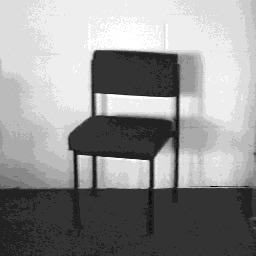
\includegraphics[width=0.22\textwidth]{img/orig/chair.jpg}}\quad
    \subfigure[Histograma]
    {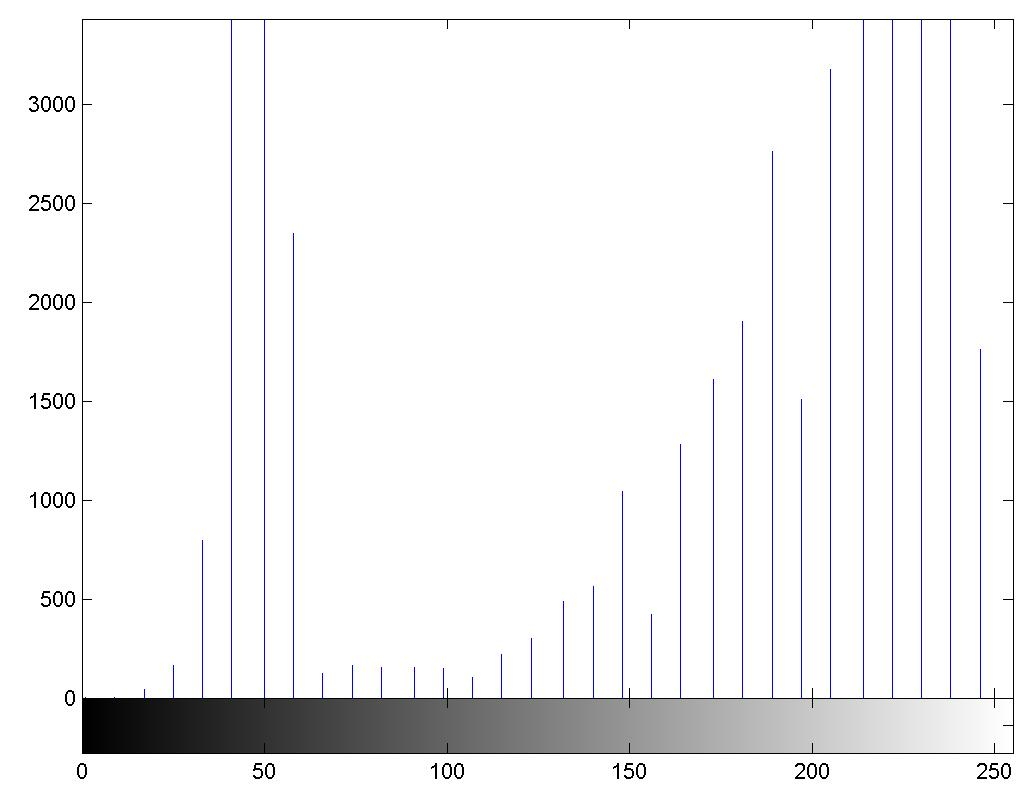
\includegraphics[width=0.28\textwidth]{img/hist/hist-chair.jpg}}\\
    \subfigure[`Bloques']    
    {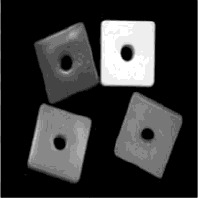
\includegraphics[width=0.22\textwidth]{img/orig/block.jpg}}\quad
    \subfigure[Umbralización del experto.]
    {
\includegraphics[width=0.22\textwidth]{img/orig/blockbin.jpg}}\quad
    \subfigure[Histrograma]
    {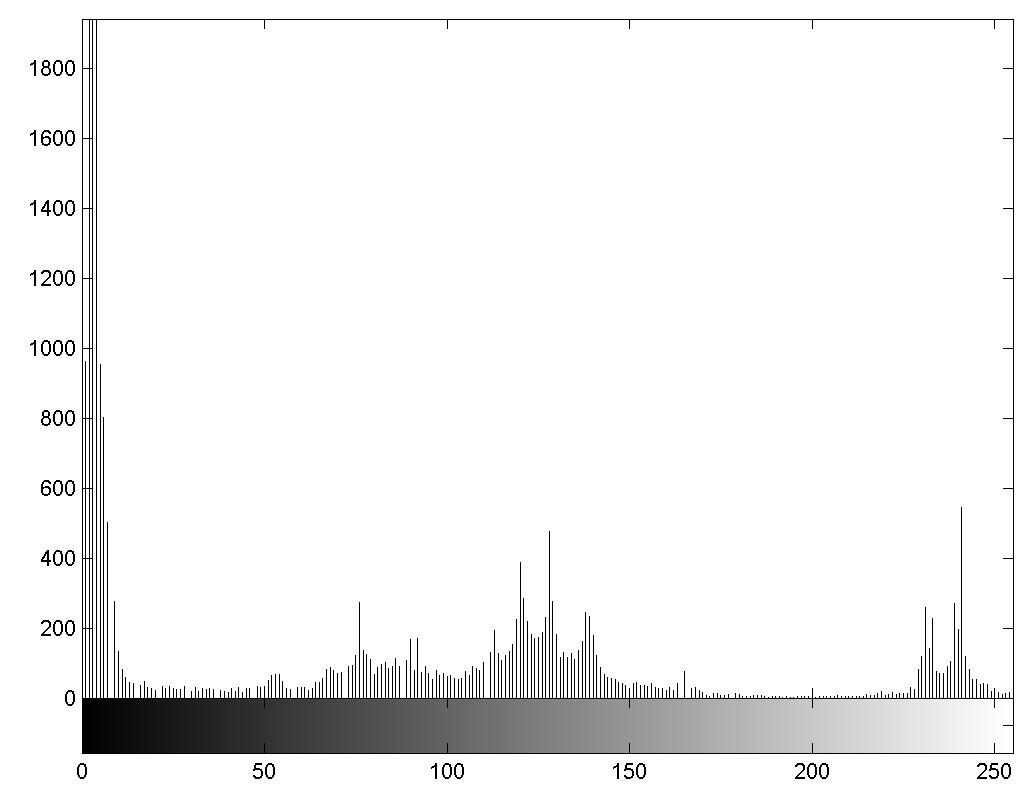
\includegraphics[width=0.28\textwidth]{img/hist/hist-block.jpg}}\\
    \subfigure[`Engranaje']
    {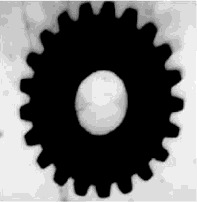
\includegraphics[width=0.22\textwidth]{img/orig/02.jpg}}\quad
    \subfigure[Umbralización del experto.]
    {
\includegraphics[width=0.22\textwidth]{img/orig/02bin.jpg}}\quad
    \subfigure[Histrograma]
    {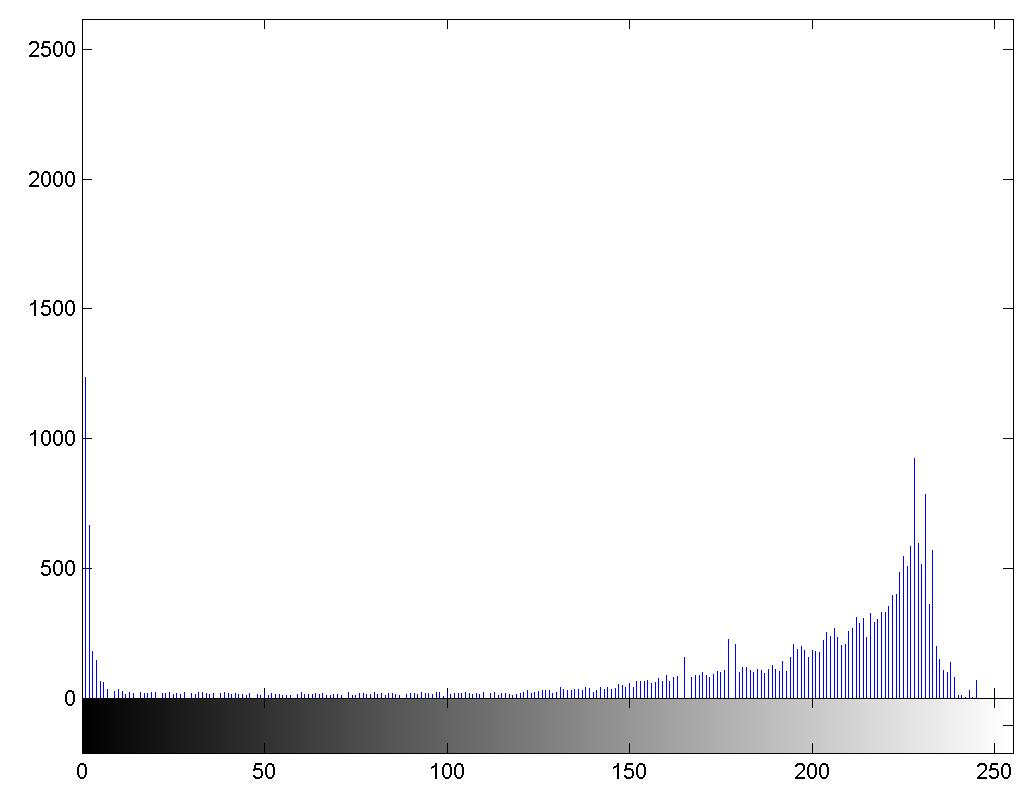
\includegraphics[width=0.28\textwidth]{img/hist/hist-02.jpg}}\\
    %\subfigure[`Piedras']
    %{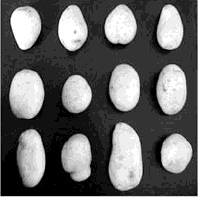
\includegraphics[width=0.22\textwidth]{img/orig/04.jpg}}\quad
    %\subfigure[Umbralización del experto.]
    %{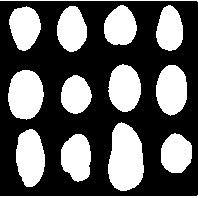
\includegraphics[width=0.22\textwidth]{img/orig/04bin.jpg}}\quad
    %\subfigure[Histrograma]
    %{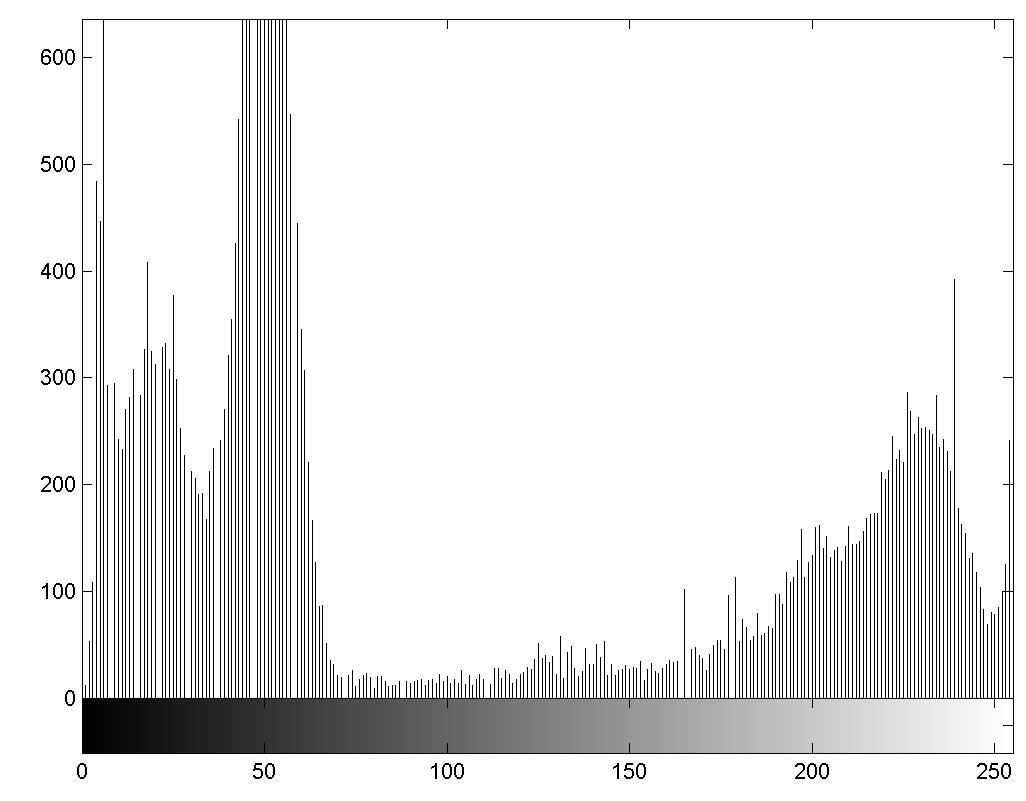
\includegraphics[width=0.28\textwidth]{img/hist/hist-04.jpg}}\\
    \subfigure[`Letras']
    {
\includegraphics[width=0.22\textwidth]{img/orig/09.jpg}}\quad
    \subfigure[Umbralización del experto.]
    {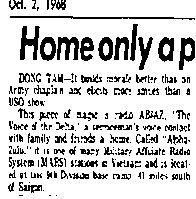
\includegraphics[width=0.22\textwidth]{img/orig/09bin.jpg}}\quad
    \subfigure[Histrograma]
    {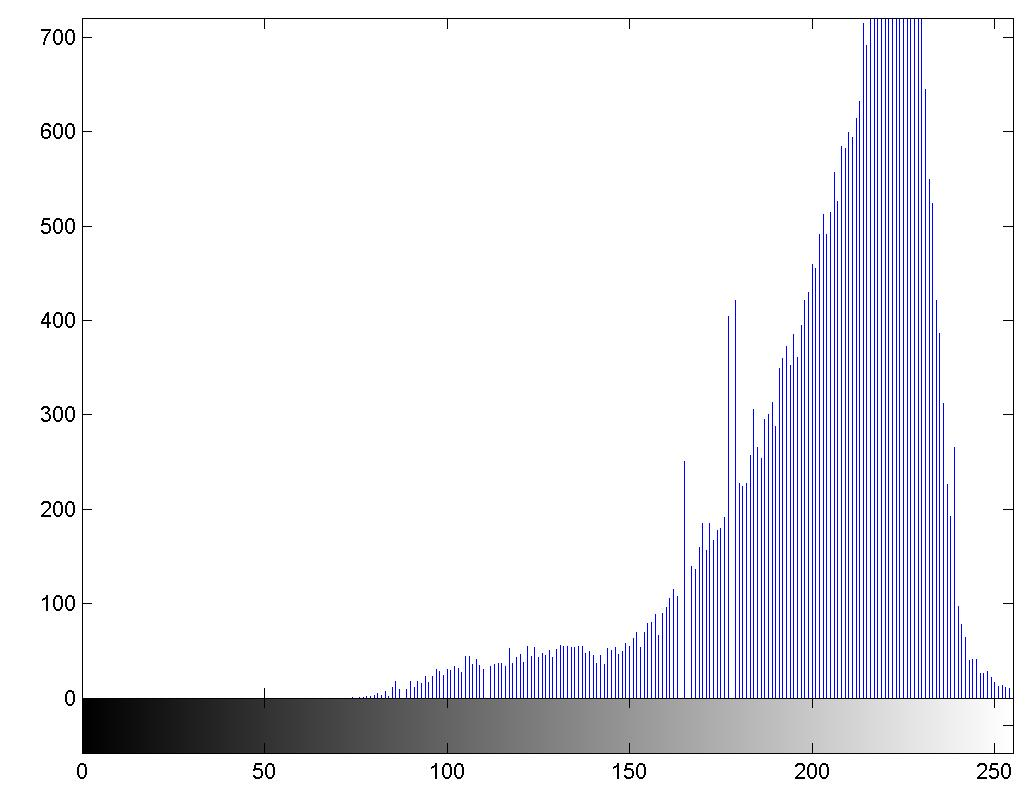
\includegraphics[width=0.28\textwidth]{img/hist/hist-09.jpg}}
    \subfigure[`Sombra']
    {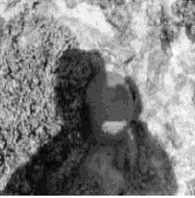
\includegraphics[width=0.22\textwidth]{img/orig/07.jpg}}\quad
    \subfigure[Umbralización del experto.]
    {
\includegraphics[width=0.22\textwidth]{img/orig/07bin.jpg}}\quad
    \subfigure[Histrograma]
    {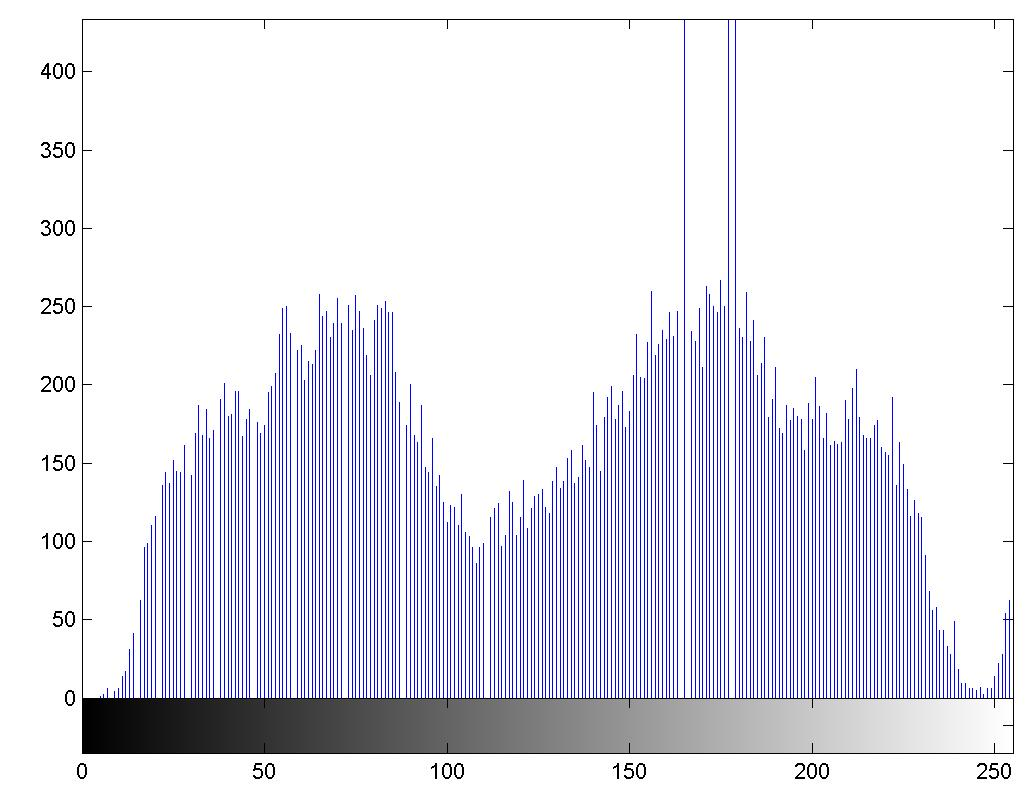
\includegraphics[width=0.28\textwidth]{img/hist/hist-07.jpg}}
    \caption{Imágenes utilizadas en el experimento 1 y siguientes.}
    \label{fig:imagenes}
\end{figure}

%\REV{faltan histogramas figura \ref{fig:sillaconruido}} Solucionado
%\REV{incluir figura con maximo contraste}
%\begin{figure}
%\centering
%    \subfigure[Muy alto contraste]
%    {\includegraphics[width=0.22\textwidth]{img/orig/chairmuyacon.jpg}}\quad
%    \subfigure[Alto contraste]
%    {\includegraphics[width=0.22\textwidth]{img/orig/chairacon.jpg}}\quad
%    \subfigure[Bajo contraste]
%    {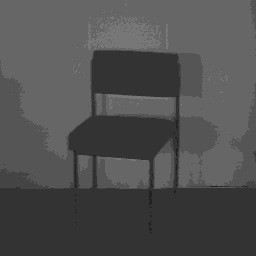
\includegraphics[width=0.22\textwidth]{img/orig/chairbcon.jpg}}\quad
%    \subfigure[Muy bajo contraste]    
%    {
\includegraphics[width=0.22\textwidth]{img/orig/chairmuybcon.jpg}}
%    \caption{Imágenes con ruido utilizadas en el experimento 1 y siguientes.}
%    \label{fig:sillaconcontraste}
%\end{figure}

\subsubsection{Resultados}
En la tabla \ref{tab:resultexp1dombi} se pueden apreciar los resultados para la umbralización de cada una de las imágenes y diferentes $w$. Se dispone, también de la tabla \ref{tab:resultexp1otros} donde se expresan los umbrales para otros algoritmos. En la comparación de ambas tablas se obtiene un resultado claro, el parámetro $w$ influye de forma determinante en la segmentación de las imágenes. Así, por ejemplo, en el caso de la `silla' $w=1$ es una opción totalmente acertada mientras que para para las `letras' habría que doblar el valor para obtener una umbralización igual de buena en comparación con los otros métodos.

\begin{table}
\centering
\begin{tabular}{c||c|c|c|c|c} 
$\mathbf{w}$    &\bb Silla&\bb Bloques&\bb Engranaje&\bb Letras&\bb Sombra\\\hline\hline
$\mathbf{0,1}$  &   218   &    255    &     250     &   142    &   200  \\\hline
$\mathbf{0,5}$  &   226   &    255    &     250     &    39    &   230  \\\hline
$\mathbf{0,75}$ &    95   &    119    &     115     &   103    &   111  \\\hline
$\mathbf{1}$    &   127   &    123    &     137     &   160    &   125  \\\hline
$\mathbf{1,25}$ &    70   &     97    &      96     &    80    &    91  \\\hline
$\mathbf{1,5}$  &    45   &     79    &      0      &    39    &    64  \\\hline
$\mathbf{2}$    &   144   &     76    &     138     &   197    &    96  \\\hline
$\mathbf{5}$    &   218   &     31    &      59     &   216    &   219  \\\hline
\end{tabular}
\caption{Umbrales para cada imagen con la función de Dombi y diferentes $w$.\label{tab:resultexp1dombi}}
\end{table}

\begin{table}
\centering
\begin{tabular}{c||c|c|c|c|c} 
                                                  &\bb Silla&\bb Bloques&\bb Engranaje&\bb Letras&\bb Sombra\\\hline\hline
\bb Alg. 1 con $\mathbf{REF_1=1-\abs{x-y}}$         &   127   &     79    &     104     &   187    &   123  \\\hline
\bb Alg. 1 con $\mathbf{REF_1=1-\abs{x-y}^2}$       &   127   &     97    &     140     &   179    &   126  \\\hline
\bb Alg. 1 con $\mathbf{REF_1=1-\abs{x-y}^{0.5}}$   &   119   &     47    &      84     &   200    &   121  \\\hline
\bb Alg. 1 con $\mathbf{REF_1=(1-\abs{x-y})^2}$     &   127   &     70    &     105     &   190    &   123  \\\hline
\bb Alg. 1 con $\mathbf{REF_1=(1-\abs{x-y})^{0.5}}$ &   127   &     82    &     104     &   186    &   124  \\\hline
\bb U. Global                                       &   130   &     79    &     105     &   187    &   124  \\\hline
\bb U. de Otsu                                      &   123   &     79    &     104     &   187    &   123  \\\hline
\bb Máx. la entropía de Renyi                       &   170   &     32    &     131     &   160    &   135  \\\hline
\end{tabular}
\caption{Umbrales para cada imagen con otras versiones de algoritmos.\label{tab:resultexp1otros}}
\end{table}

Por otra parte, cabe destacar que este resultado se ha obtenido en un tiempo de computación de alrededor de 0,0025 segundos, tanto para la versión con función de Dombi como para la de REF. Con la intención de que el lector pueda juzgar adecuadamente estos resutlados, se presentan los resultados, en forma gráfica, para aquellos valores de $w$ más reelevantes de forma gráfica en la tabla \ref{tab:resultexp1imagenesdombi}. Se facilita la posibilidad de poder compararlo directamente con el algoritmo original. Además, se dispone en el apéndice, en la tabla \ref{tab:otrassegmentaciones}, la umbralización de las imágenes con otros algoritmos para que se pueda llevar a cabo también la comparación.

\begin{table}
\centering
\begin{tabular}{c||c|c|c} 
$\mathbf{REF_1=1-\abs{x-y}}$ & $\mathbf{w=0,75}$ &\bb $\mathbf{w=1}$ &\bb $\mathbf{w=1,25}$\\\hline\hline
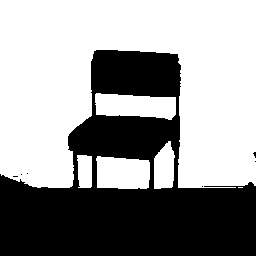
\includegraphics[width=0.2\textwidth]{img/res/e1a/alg1tipo1-chair.jpg} &
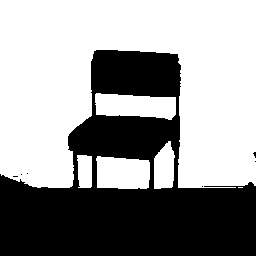
\includegraphics[width=0.2\textwidth]{img/res/e1a/alg1tipo6-chair.jpg} &

\includegraphics[width=0.2\textwidth]{img/res/e1a/alg1tipo6d0.75-chair.jpg} &
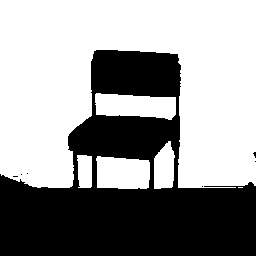
\includegraphics[width=0.2\textwidth]{img/res/e1a/alg1tipo6d1.25-chair.jpg} \\
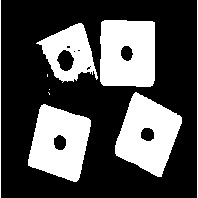
\includegraphics[width=0.2\textwidth]{img/res/e1a/alg1tipo1-block.jpg} &

\includegraphics[width=0.2\textwidth]{img/res/e1a/alg1tipo6-block.jpg} &
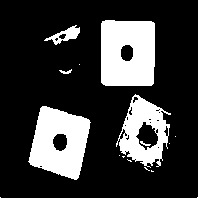
\includegraphics[width=0.2\textwidth]{img/res/e1a/alg1tipo6d0.75-block.jpg} &

\includegraphics[width=0.2\textwidth]{img/res/e1a/alg1tipo6d1.25-block.jpg} \\

\includegraphics[width=0.2\textwidth]{img/res/e1a/alg1tipo1-02.jpg} &

\includegraphics[width=0.2\textwidth]{img/res/e1a/alg1tipo6-02.jpg} &

\includegraphics[width=0.2\textwidth]{img/res/e1a/alg1tipo6d0.75-02.jpg} &

\includegraphics[width=0.2\textwidth]{img/res/e1a/alg1tipo6d1.25-02.jpg} \\
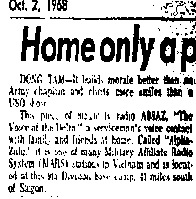
\includegraphics[width=0.2\textwidth]{img/res/e1a/alg1tipo1-09.jpg} &
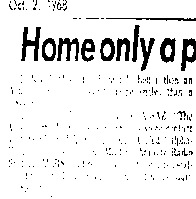
\includegraphics[width=0.2\textwidth]{img/res/e1a/alg1tipo6-09.jpg} &

\includegraphics[width=0.2\textwidth]{img/res/e1a/alg1tipo6d0.75-09.jpg} &
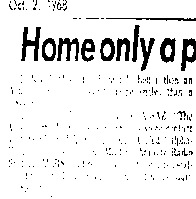
\includegraphics[width=0.2\textwidth]{img/res/e1a/alg1tipo6d1.25-09.jpg} \\
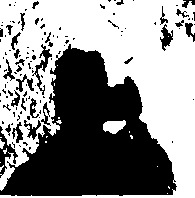
\includegraphics[width=0.2\textwidth]{img/res/e1a/alg1tipo1-07.jpg} &

\includegraphics[width=0.2\textwidth]{img/res/e1a/alg1tipo6-07.jpg} &

\includegraphics[width=0.2\textwidth]{img/res/e1a/alg1tipo6d0.75-07.jpg} &

\includegraphics[width=0.2\textwidth]{img/res/e1a/alg1tipo6d1.25-07.jpg} \\\hline
\end{tabular}
\caption{Resultado de las segmentaciones para el algoritmo con REF y Dombi con varios $w = \{0,75; 1; 1,25\}$.\label{tab:resultexp1imagenesdombi}}
\end{table}

Para poder comprobar y comparar formalmente todos los resultados, se calcula el error cuadrático medio para las imágenes. En concreto, se hace con todas las versiones obtenidas con otros los algoritmos presentados sin obtener ningún resultado reelevante. Se presentan en la tabla \ref{tab:erroresexp1dombi}, la comparación que se hace entre las segmentaciones que se obtienen con varias $w$ y la imagen umbralizada de forma exacta por un experto, resultados que se hacen más interesantes que los anteriores. De nuevo, de esta tabla se desprende de que en función de la imagen que se tome, el parámetro $w$ para obtener una mejor umbralización.

\begin{table}
\centering
\begin{tabular}{c||c|c|c|c} 
$\mathbf{w}$                    &\bb Bloques&\bb Engranaje&\bb Letras&\bb Sombra\\\hline\hline
\bb Alg. 1 con $\mathbf{0,75}$  &   43,3750  &   33,0080   &   33,3617   &   59,2420  \\\hline
\bb Alg. 1 con $\mathbf{1}$     &   49,8760  &   36,3914   &   29,6418   &   52,0672  \\\hline
\bb Alg. 1 con $\mathbf{1,25}$  &   50,0241  &   32,0153   &   31,0001   &   55,0322  \\\hline
\end{tabular}
\caption{Errores para las imágenes con ruido con otras versiones de algoritmos.\label{tab:erroresexp1dombi}}
\end{table}


%Con ruido
Con la intención de poder llevar a cabo experimentos sobre imágenes con ruido, se crean estas de forma sintética, tal y como se ha presentando en la sección \ref{sec:ruido}. Se pueden ver los resultados sobre la imagen `silla', y sus histogramas, en la figura \ref{fig:imagenesruido}. 

\begin{figure}
\centering
    \subfigure[Ruido gausiano]
    {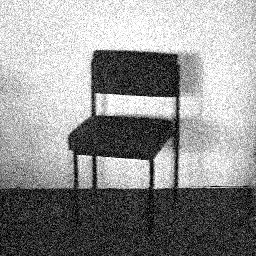
\includegraphics[width=0.25\textwidth]{img/orig/chairga.jpg}}\quad
    \subfigure[Ruido `sal y pimienta' con $p=0,05$]
    {
\includegraphics[width=0.25\textwidth]{img/orig/chairs&p005.jpg}}\quad
    \subfigure[Ruido `sal y pimienta' con $p=0,2$]    
    {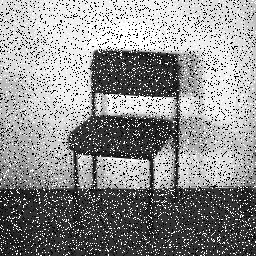
\includegraphics[width=0.25\textwidth]{img/orig/chairs&p020.jpg}}
    \subfigure[Histograma de ruido gausiano]
    {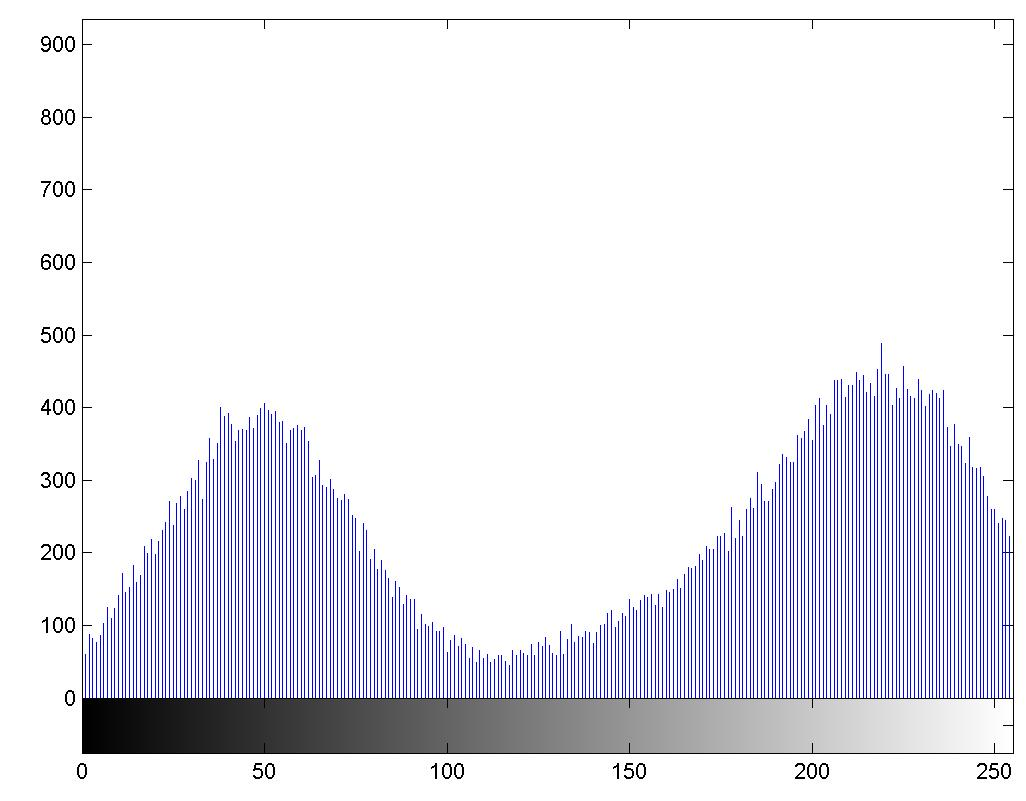
\includegraphics[width=0.3\textwidth]{img/hist/hist-chairga.jpg}}\quad
    \subfigure[Histograma de ruido `sal y pimienta' con $p=0,05$]
    {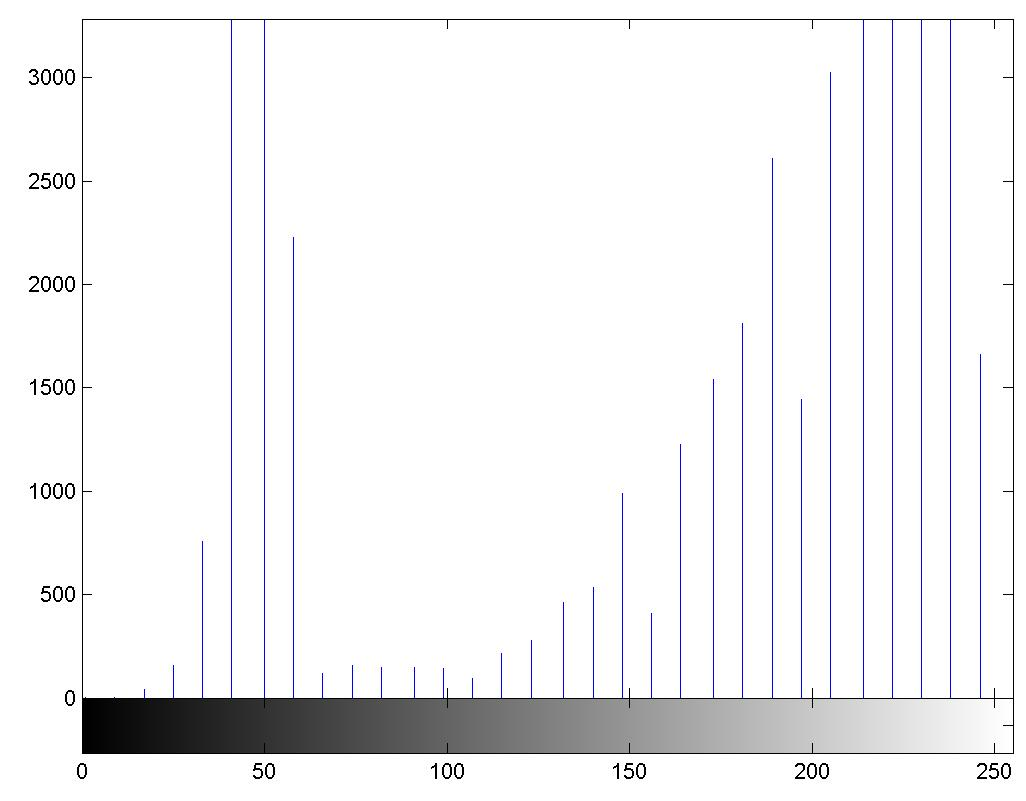
\includegraphics[width=0.3\textwidth]{img/hist/hist-chairsp005.jpg}}\quad
    \subfigure[Histograma de ruido `sal y pimienta' con $p=0,2$]    
    {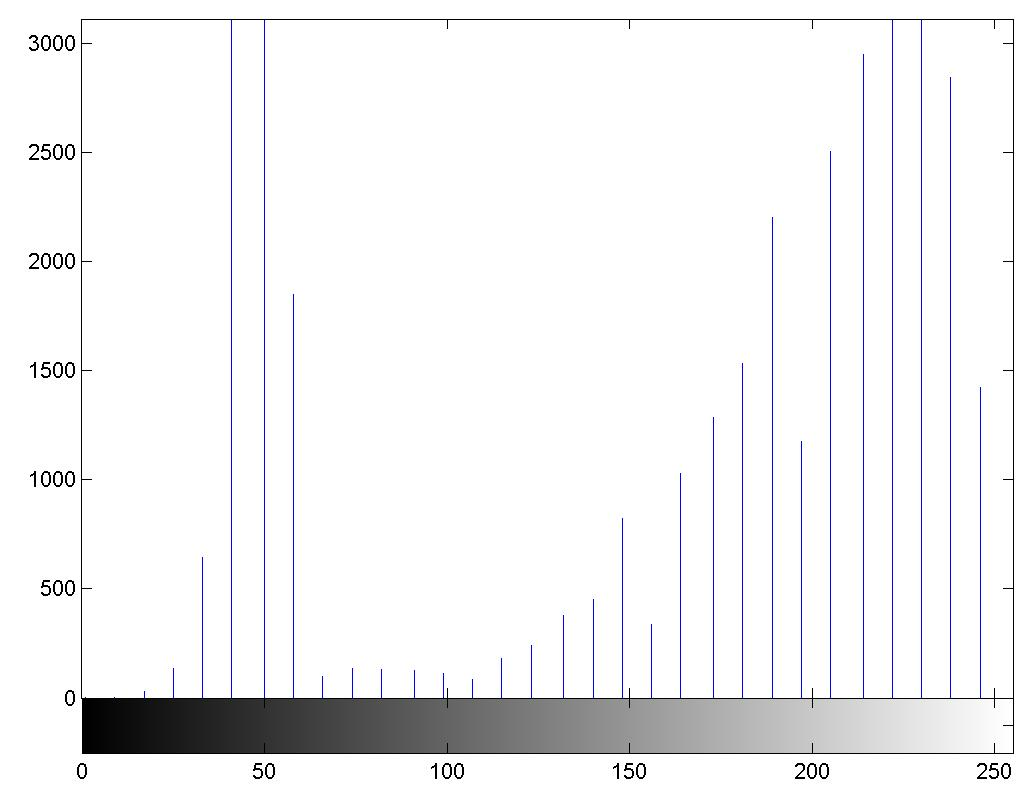
\includegraphics[width=0.3\textwidth]{img/hist/hist-chairsp020.jpg}}
    \caption{Imágenes con ruido utilizadas en el experimento 1 y siguientes.}
    \label{fig:imagenesruido}
\end{figure}

Los umbrales que se han obtenido se expresan en la tabla \ref{tab:resultexp1ruido}. Comparándola de nuevo con otros algoritmos (tablas \ref{tab:resultexp1ruidootros}), se puede apreciar que se pueden obtener resultados similiares también e, igualmente, que el parámetro $w$ es decisivo para diferentes imágenes. Es curioso comprobar el hecho de que con la misma $w$ se obtienen resultados similares en comparación con los umbrales de la versión original con REF. 

\begin{table}
\centering
\begin{tabular}{c||c|c|c} 
           &\bb R. gausiano&\bb R. impulsivo 0.05&\bb R. impulsivo 0.2\\\hline\hline
$\mathbf{0,1}$  &   219   &    226    &     226     \\\hline
$\mathbf{0,5}$  &   234   &    226    &     242     \\\hline
$\mathbf{0,75}$ &    99   &     95    &      95     \\\hline
$\mathbf{1}$    &   128   &    127    &     127     \\\hline
$\mathbf{1,25}$ &    74   &     70    &      62     \\\hline
$\mathbf{1,5}$  &    35   &     45    &      37     \\\hline
$\mathbf{2}$    &   147   &    136    &     127     \\\hline
$\mathbf{5}$    &   226   &    218    &     226     \\\hline
\end{tabular}
\caption{Umbrales para las imágenes con ruido con la función de Dombi y diferentes valores de $w$.\label{tab:resultexp1ruido}}
\end{table}


\begin{table}
\centering
\begin{tabular}{c||c|c|c} 
                          &\bb R. gausiano&\bb R. impulsivo 0.05&\bb R. impulsivo 0.2\\\hline\hline
\bb Alg. 1 con $\mathbf{REF_1=1-\abs{x-y}}$             &   132   &    127    &     127     \\\hline
\bb Alg. 1 con $\mathbf{REF_1=1-\abs{x-y}^2}$           &   131   &    127    &     127     \\\hline
\bb Alg. 1 con $\mathbf{REF_1=1-\abs{x-y}^{0.5}}$       &   131   &    136    &     152     \\\hline
\bb Alg. 1 con $\mathbf{REF_1=(1-\abs{x-y})^2}$         &   132   &    127    &     127     \\\hline
\bb Alg. 1 con $\mathbf{REF_1=(1-\abs{x-y})^{0.5}}$     &   131   &    127    &     127     \\\hline
\bb U. Global                                           &   132   &    130    &     128     \\\hline
\bb U. de Otsu                                          &   132   &    123    &     123     \\\hline
\bb Máx. la entropía de Renyi                           &   154   &    170    &     170     \\\hline
\end{tabular}
\caption{Umbrales para las imágenes con ruido con otras versiones de algoritmos.\label{tab:resultexp1ruidootros}}
\end{table}

En cuanto al tiempo de cómputo, de nuevo vuelven a estar todos los valores entorno a 0,0025 segundos. Esto hace ver que el método presentado sigue siendo igual de eficiente que la versión original. Así mismo, se muestran los resultados gráficamente en la tabla \ref{tab:resultexp1imagenesruido}.

\begin{table}
\centering
\begin{tabular}{c||c|c|c} 
$\mathbf{REF_1=1-\abs{x-y}}$ & $\mathbf{w=0,75}$ &\bb $\mathbf{w=1}$ &\bb $\mathbf{w=1,25}$\\\hline\hline
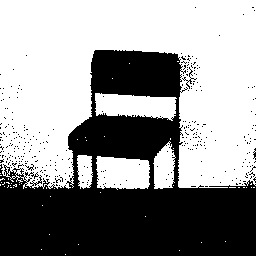
\includegraphics[width=0.2\textwidth]{img/res/e1a/alg1tipo1-chairga.jpg} &
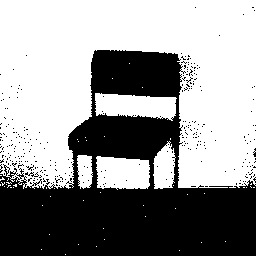
\includegraphics[width=0.2\textwidth]{img/res/e1a/alg1tipo6-chairga.jpg} &

\includegraphics[width=0.2\textwidth]{img/res/e1a/alg1tipo6d0.75-chairga.jpg} &
\includegraphics[width=0.2\textwidth]{img/res/e1a/alg1tipo6d1.25-chairga.jpg} \\
\includegraphics[width=0.2\textwidth]{img/res/e1a/alg1tipo1-chairsp005.jpg} &
\includegraphics[width=0.2\textwidth]{img/res/e1a/alg1tipo6-chairsp005.jpg} &
\includegraphics[width=0.2\textwidth]{img/res/e1a/alg1tipo6d0.75-chairsp005.jpg} &
\includegraphics[width=0.2\textwidth]{img/res/e1a/alg1tipo6d1.25-chairsp005.jpg} \\
\includegraphics[width=0.2\textwidth]{img/res/e1a/alg1tipo1-chairsp020.jpg} &
\includegraphics[width=0.2\textwidth]{img/res/e1a/alg1tipo6-chairsp020.jpg} &
\includegraphics[width=0.2\textwidth]{img/res/e1a/alg1tipo6d0.75-chairsp020.jpg} &
\includegraphics[width=0.2\textwidth]{img/res/e1a/alg1tipo6d1.25-chairsp020.jpg} \\\hline
\end{tabular}
\caption{Umbrales para las imágenes con ruido con otras versiones de algoritmos.\label{tab:resultexp1imagenesruido}}
\end{table}

En relación con los errores con imagenes umbralizadas con otros algoritmos, no se obtiene ningún resultado concluyente ya que en ningún momento el error pasa de 0,1.

Además, se han hecho experimentos con imágenes con mucho y poco contraste. En este caso, la solución tenía el error de nuevo en un rango de diferencia de una décima, aunque permite llegar a opciones con mucho más bajo contraste que el algoritmo de la maximización de la entropía de Renyi, que es el que mejor lo hace entre los otros algoritmos presentados. En definitiva, con el algoritmo de maximización de la similitud se pueden llegar a segmentar imágenes con intervalos de menos de 15 niveles de gris. Se encuentra, también, el hechod de que en el caso de crear dos imágenes con alto y bajo contraste que sean ``contrarias'', la segmentación que se obtiene es la misma.


% EXPERIMENTO 2
\subsection{Experimento 2: busqueda del mejor umbral a través de funciones penalti\label{sec:exp2}}
\subsubsection{Explicación del experimento}
En vista del experimento anteior donde había momentos en los que la función de dombi no actuaba de forma correcta, se propone una nueva forma para poder elegir entre la función de Dombi o volver al método con la función REF. En concreto, se intentará dilucidar esta situación por medio de una función penalti. El proceso de la obtención del conjunto difuso cambiará, ya que no será una única función y tendrá el siguiente orden:
\begin{enumerate}
    \item Creación de todas las pertenencias con las 5 funciones REF presentadas y la función de Dombi con $w=1$.
    \item Agregación de todas las pertenencias anteriores con varias funciones, a saber:
        \begin{enumerate}
            \item Media aritmética.
            \item Media geométrica.
            \item Máximo.
            \item Mínimo.
            \item Integral Choquet.
            \item OWA de `al menos la mitad'. %\REV{nombre}
        \end{enumerate}    
    \item Con todos estos resultados se actua con la función penalti para cada uno de los elementos $a_1,\dots a_n$ agregados y las pertenencias obtenidas en (1) $r=(r_1,\dots, r_m)$, obtendremos $p(a_i, r)=\sum_{j=1}^m \abs{a_i-r_j}$.
    \item Cogeremos como pertenencia aquel resultado de la agregación, $a_i$, que haga que el resultado de la función penalti sea máximo.  
\end{enumerate}

En vista de que los resultados de la idea presentada anteriormente no presentaba a penas diferencia con el experimento 1. Por esta razón, en una segunda versión, se añadirá también la función de agregación siguiente con la intención de crear más {\em outlayers} que creen más posibles umbrales.
$$M_{zadeh}(r_1,\dots,r_m)=\max\left(0, \sum r-(n-1)\right)\cdot \sqrt[n]{\prod_{i=1}^n{r_i}}$$
Esta segunda versión son los resultados que se presentan a continuación.

\subsubsection{Resultados}

En la tabla \ref{tab:resultexp2agregado} se recogen los umbrales $t$ creados a través de la función penalti. De nuevo, en comparación con los presentados en la tabla \ref{tab:resultexp1otros} se puede observar que siempre son valores que se encuentran en el intervalo que pueden definir. Esto hace suponer que las imágenes tiene una umbralización correcta, algo que se puede comprobar con las imágenes del cuadro \ref{tab:resultexp2imagenagregado}. En relación al error (tabla \ref{tab:resultexp2agregado})sorprende la diferencia que existe frente

\begin{table}
\centering
\begin{tabular}{c|c|c|c|c} 
\bb Silla&\bb Bloques&\bb Engranaje&\bb Letras&\bb Sombra\\\hline\hline
   127   &     68    &      92     &   196    &   123  \\\hline
\end{tabular}
\caption{Umbrales para cada imagen con el algoritmo 1 calculando la función de pertenencia a través de una función penalti.\label{tab:resultexp2agregado}}
\end{table}


\begin{table}
\centering
\begin{tabular}{ccccc}\hline
\includegraphics[width=0.15\textwidth]{img/res/e2a/alg1agregate-chair.jpg} &
\includegraphics[width=0.15\textwidth]{img/res/e2a/alg1agregate-block.jpg} &
\includegraphics[width=0.15\textwidth]{img/res/e2a/alg1agregate-02.jpg} &
\includegraphics[width=0.15\textwidth]{img/res/e2a/alg1agregate-09.jpg} &
\includegraphics[width=0.15\textwidth]{img/res/e2a/alg1agregate-07.jpg}\\\hline
\end{tabular}
\caption{Resultado para el nuevo algoritmo a través de penalti con todas las funciones propuestas.\label{tab:resultexp2imagenagregado}}
\end{table}


\begin{table}
\centering
\begin{tabular}{c|c|c|c|c} 
\bb Bloques&\bb Engranaje&\bb Letras&\bb Sombra\\\hline\hline
     90,3727    &      124,9112     &     140,5241    &     194,3489  \\\hline
\end{tabular}
\caption{Errores en comparación con las imágenes segmentadas por el experto.\label{tab:erroresexp2agregado}}
\end{table}


Además, en la tabla \ref{tab:resultexp2agregadoruido} se pueden observar los umbrales obtenidos para las imágenes con ruido. De forma similar a las imágenes normales, el umbral vuelve a estar en el intervalo que se crea con los umbrales originales del experimento anterior. Tal y como se puede ver en la tabla \ref{tab:resultexp2imagenagregadoruido} el resultado para las imágenes con ruido gausiano y con ruido `sal y pimienta' con $p=0,05$ mientras que subiendo la probabilidad para el ruido, el umbral comienza a ser bastante inadecuado. Como es lógico, el ruido impulsivo no se consigue resolver aunque tampoco es así en el caso del gausiano, que segmenta de forma bastante adecuada aun no apreciandose un mínimo claro.

\begin{table}
\centering
\begin{tabular}{c|c|c} 
\bb R. gausiano&\bb R. impulsivo 0.05&\bb R. impulsivo 0.2\\\hline\hline
   132   &     127    &      152    \\\hline
\end{tabular}
\caption{Umbrales para cada imagen ruido a través del algoritmo 1 calculando la función de pertenencia a través de una función penalti.\label{tab:resultexp2agregadoruido}}
\end{table}


\begin{table}
\centering
\begin{tabular}{ccc}\hline
\includegraphics[width=0.2\textwidth]{img/res/e2a/alg1agregate-chairga.jpg} &
\includegraphics[width=0.2\textwidth]{img/res/e2a/alg1agregate-chairsp005.jpg} &
\includegraphics[width=0.2\textwidth]{img/res/e2a/alg1agregate-chairsp020.jpg}\\\hline
\end{tabular}
\caption{Resultado para el nuevo algoritmo a través de penalti con todas las funciones propuestas para imágenes con ruido.\label{tab:resultexp2imagenagregadoruido}}
\end{table}



% EXPERIMENTO 3
\subsection{Experimento 3: sustitución de la función REF por la función de Dombi en el algoritmo para la obtenición del umbral óptimo}

\subsubsection{Explicación del experimento}
En este experimento se ha tomado el algoritmo de obtención del umbal óptimo maximizando la similitud (algoritmo 3A) para comprobar el efecto de la función de Dombi en él. Por esta razón, y en vista de los resultados del experimento 1, se plantean dos variantes. En primer lugar, se incorpora la función de dombi a las 5 funciones REF que ya estaban para poder ver qué umbral se obtiene, intentando escoger el mejor (algoritmo 3B). Después, se eligen los diferentes valores de $w$ que se han utilizado antes (algoritmo 3C). De esta forma, se intenta buscar cual de los umbrales calculados anteriormente de forma individual es el mejor.

\subsubsection{Resultados}

Hecho todo el cómputo, en la tabla \ref{tab:resultexp3dombi} se muestran los umbrales obtenidos tanto con el algoritmo original como por parte de las dos versiones que se han propuesto. Por un lado, es muy visible el hecho de que para la mayor parte de las imágenes la versión C no tiene utilidad, ya que elige umbrales totalmente fuera de la lógica. Por otra parte, se ve que la versión B es muy similar a la versión original. Esto hace pensar que esta versión podría hacer que las funciones de Dombi fueran interesantes para algunos casos. Los resultados gráficos se presentan en la tabla \ref{tab:resultexp3imagenesdombi}

\begin{table}
\centering
%\resizebox*{3\textwidth}{!}{
\begin{tabular}{c||c|c|c|c|c} 
             &\bb Silla&\bb Bloques&\bb Engranaje&\bb Letras&\bb Sombra\\\hline\hline
\bb Alg. 3A  &   115   &    80    &     88      &    199   &    121   \\\hline
\bb Alg. 3B  &   127   &    123    &     84      &    200   &    125   \\\hline
\bb Alg. 3C  &   218   &    254    &     250     &    142   &    219   \\\hline
\end{tabular}
\caption{Umbrales para cada imagen con el algoritmo 3 en todas sus nuevas versiones.\label{tab:resultexp3dombi}}
\end{table}


\begin{table}
\centering
\begin{tabular}{cccccc}\hline
Alg. 3B\quad
\includegraphics[width=0.15\textwidth]{img/res/e3a/alg3btipo-chair.jpg} &
\includegraphics[width=0.15\textwidth]{img/res/e3a/alg3btipo-block.jpg} &
\includegraphics[width=0.15\textwidth]{img/res/e3a/alg3btipo-02.jpg} &
\includegraphics[width=0.15\textwidth]{img/res/e3a/alg3btipo-09.jpg} &
\includegraphics[width=0.15\textwidth]{img/res/e3a/alg3btipo-07.jpg}\\\hline
Alg. 3C\quad     
\includegraphics[width=0.15\textwidth]{img/res/e3a/alg3ctipo-chair.jpg} &
\includegraphics[width=0.15\textwidth]{img/res/e3a/alg3ctipo-block.jpg} &
\includegraphics[width=0.15\textwidth]{img/res/e3a/alg3btipo-02.jpg} &
\includegraphics[width=0.15\textwidth]{img/res/e3a/alg3ctipo-09.jpg} &
\includegraphics[width=0.15\textwidth]{img/res/e3a/alg3ctipo-07.jpg}\\\hline
\end{tabular}
\caption{Resultado gráfico con el algoritmo 3 con las nuevas propuestas.\label{tab:resultexp3imagenesdombi}}
\end{table}

En cuanto al tiempo de cómputo, aunque crece con respecto a los algoritmos de los experimentos anteriores, este sigue estando en la misma media del algoritmo original, siempre que se tome como versión original la que definen las 5 REF del algoritmo 1. Todos los resultados gráficos son resumidos en la tabla \ref{tab:resultexp3imagenesdombi}.

%\REV{errores, imposible que sean esos...}

Para poder conocer cómo de buenos son los resultados, se comparan las imágenes obteniendo el error cuadrático medio (tabla\ref{tab:erroresexp3otros}). En esta se puede apreciar cómo se mantiene un error bastante similar con todos los algoritmos.

%\begin{table}
%\centering
%\begin{tabular}{c||c|c|c|c}
%                &\bb Bloques  &\bb Engranaje&\bb Letras  &\bb Sombra  \\\hline\hline
%\bb Alg. 3B     &   0,0082   &   124,9112   &   0,2019   &   0,1017   \\\hline
%\bb Alg. 3C     &     0      &   124,9112   &   0,0136   &   0,5744   \\\hline
%\end{tabular}
%\caption{Errores de las imágenes perfectas para cada imagen con el algoritmo 3 en todas sus versiones.\label{tab:erroresexp3dombi}}
%\end{table}


\begin{table}
\centering
\begin{tabular}{c||c|c|c|c}
                        &\bb Silla    &\bb Bloques  &\bb Engranaje &\bb Sombra    \\\hline\hline
\bb Alg. 3A (Original)  &   72,8822   &   93,8135   &   126,5836   &   124,7987   \\\hline
\bb Umb. Global         &   71,7070   &   81,0453   &   124,7637   &   122,4343   \\\hline
\bb {\em K-means}       &   71,7070   &   81,0453   &   124,9112   &   123,2863   \\\hline
\bb Método de Otsu      &   71,7070   &   81,0453   &   124,9112   &   123,2863   \\\hline
\bb Máx. Entropía Renyi &   56,9290   &   96,4543   &   121,5597   &   112,4747   \\\hline
\end{tabular}
\caption{Erorres de las imágenes obtenidas con otros algoritmos para cada imagen con el algoritmo 3 en todas sus versiones.\label{tab:erroresexp3otros}}
\end{table}


Se comprueba que las tendencias anteriores son también seguidas por aquellas imágenes que disponen de ruido. Es decir, la versión que se propone con la función de dombi con diferentes valores de $w$. También, los resultados con la versión B son más bajos con respecto a las versión original, algo que como se ha visto es bastante común desde el momento en el que se introducen las funciones de Dombi.


\begin{table}
\centering
\begin{tabular}{c||c|c|c}
        &\bb R. gausiano&\bb R. impulsivo 0.05&\bb R. impulsivo 0.2\\\hline\hline
\bb Alg. 3A  &   131   &    136    &     144      \\\hline
\bb Alg. 3B  &   128   &    127    &     127      \\\hline
\bb Alg. 3C  &   226   &    218    &     226      \\\hline
\end{tabular}
\caption{Umbrales para cada imagen ruidosa con el algoritmo 3 en todas sus versiones.\label{tab:resultexp3ruido}}
\end{table}



\begin{table}
\centering
\begin{tabular}{cccccc}\hline
Alg. 3B\quad
\includegraphics[width=0.18\textwidth]{img/res/e3a/alg3btipo-chairga.jpg} &
\includegraphics[width=0.18\textwidth]{img/res/e3a/alg3btipo-chairsp005.jpg} &
\includegraphics[width=0.18\textwidth]{img/res/e3a/alg3btipo-chairsp020.jpg}\\\hline
Alg. 3C\quad     
\includegraphics[width=0.18\textwidth]{img/res/e3a/alg3ctipo-chairga.jpg} &
\includegraphics[width=0.18\textwidth]{img/res/e3a/alg3ctipo-chairsp005.jpg} &
\includegraphics[width=0.18\textwidth]{img/res/e3a/alg3ctipo-chairsp020.jpg}\\\hline
\end{tabular}
\caption{Representación gráfica del resultado .\label{tab:resultexp3imagenesruido}}
\end{table}


\begin{table}
\centering
\begin{tabular}{c||c|c|c}
        &\bb R. gausiano&\bb R. impulsivo 0.05&\bb R. impulsivo 0.2\\\hline\hline
\bb Alg. 3 Original     &   95,1075   &   66,4737   &   74,2907   \\\hline
\bb Umb. Global         &   94,8740   &   68,2635   &   77,5124   \\\hline
\bb {\em K-means}       &   95,1074   &   68,2635   &   77,5124   \\\hline
\bb Método de Otsu      &   94,8740   &   68,2635   &   77,5124   \\\hline
\bb Máx. Entropía Renyi &   85,9364   &   54,1976   &   65,7772   \\\hline
\end{tabular}
\caption{Errores para cada imagen ruidosa con otros algoritmos tomando como referencia la versión 3B.\label{tab:erroresexp3ruido}}
\end{table}



\subsection{Repetición de los experimentos con la corrección oportuna.}\label{sec:cambiodombi}
Vistos los resultados de los experimentos anteriores, y en especial el que se refiere al experimento 3, se plantea el porqué se obtiene un resultado tan malo. Este hecho es extraño sobre todo por el hecho de que a través de los diferentes valores de $w$, el algoritmo 1 con las funciones de dombi siempre tiene buenos resultados. Se comprueba el vector de similitudes que se obtiene para dilucidar qué umbral escoger en el algoritmo 3, lo que muestra que la similitud mayor no se encuentra en el mejor umbral. %\REV{¿ejemplo?}

Reestudiando la situación, se encuentra que en las propiedades de las funciones que propone Dombi (Lema \ref{def:propiedadesdombi}) se ha omitido que una función de equivalencia $e$ cumple $e(x,x)=1$. En particular, las funciones REF son un ejemplo de esta situación. La razón por la que no se puede cumplir esta propiedad es porque existe otra que dice $e(x,n(x))=0$. Como es evidente, el intentar mantener ambas a la vez es una contradicción. Por esta razón, el autor dice que sus funciones cumplirán en parte ambas en función de un parámetro. Esto hace que para dos elementos iguales no tengamos como resultado 1. 

Vista la situación y sabiendo que la construcción que se utiliza para los conjuntos difusos hace necesario que la condición anterior se cumpla de forma plena, se intenta reescribir la función de pertenencia a los conjuntos difusos. De esta forma, se aplica a todos los experimentos que se han mostrado anteriormente esta nueva función (ecuación \ref{eq:intentodesolucionardombi})

\begin{equation}\label{eq:intentodesolucionardombi}
    \mu_{Q_t}(q)=\left\{ \begin{split}
                 \min\left( 1, \frac
                    {\unmedio \left(1+\left(1-\frac{2q}{L-1}\right)\left(1-\frac{2m_b}{L-1}\right)\right)}
                    {\unmedio \left(1+\left(1-\frac{2m_b}{L-1}\right)\left(1-\frac{2m_b}{L-1}\right)\right)}\right)
                 \text{\quad si\quad} q\leq t\\
                 \min\left( 1, \frac
                    {\unmedio \left(1+\left(1-\frac{2q}{L-1}\right)\left(1-\frac{2m_o}{L-1}\right)\right)}
                    {\unmedio \left(1+\left(1-\frac{2m_o}{L-1}\right)\left(1-\frac{2m_o}{L-1}\right)\right)}\right)
                \text{\quad si\quad} q > t
                \end{split}\right.
\end{equation}



%RESULTADOS DE LA REESCRITURA
\subsubsection{Resultados}
La opción que se ha propuesto anteriormente ha tenido resultados muy malos, de hecho, mucho peores que las presentadas en las secciones anteirores. Por esa razón y únicamente a modo de ejemplo, en las tablas \ref{tab:resultexp1bdombi} y \ref{tab:resultexp3bdombi} se pueden ver algunos resultados obtenidos. Este algoritmo, es por tanto, desechado de forma completa. Se acaba concluyendo que las funciones de Dombi no pueden sustituir directamente a funciones REF tal y como el autor sugería. Por esta razón, la umbralización con los métodos anteriores presentará resultados hetereogéneos lo que hace que no sea un método útil para su utilización habitual.

\begin{table}\begin{center}
%\resizebox*{3\textwidth}{!}{
\begin{tabular}{cc||c|c|c|c|c} 
                                    &                   &\bb Silla&\bb Bloques&\bb Engranaje&\bb Letras&\bb Sombra\\\hline\hline
\bb{\multirow{2}{1.75cm}{$w=0,1$}}  &  \bb Umbral ($t$) &   234   &     8     &      0      &   157    &   250  \\
                                    &  \bb Tiempo (s)   &  0,002  &   0,675   &    0,686    &  0,689   &  0,688 \\\hline
\bb\multirow{2}{1.75cm}{$w=0,5$}    &  \bb Umbral ($t$) &   226   &     8     &     111     &   207    &   254  \\
                                    &  \bb Tiempo (s)   &  0,002  &   0,649   &    1,093    &  1,233   &  1,13  \\\hline
\bb\multirow{2}{1.75cm}{$w=0,75$}   &  \bb Umbral ($t$) &   226   &     8     &     122     &   182    &   238  \\
                                    &  \bb Tiempo (s)   &  0,002  &   0,677   &    0,686    &  0,688   &  0,679 \\\hline
\bb\multirow{2}{1.75cm}{$w=1$}      &  \bb Umbral ($t$) &   226   &     8     &      90     &   191    &   246  \\
                                    &  \bb Tiempo (s)   &  0,002  &   0,63    &    0,642    &  0,646   &  0,642 \\\hline
\bb\multirow{2}{1.75cm}{$w=1,25$}   &  \bb Umbral ($t$) &   226   &     8     &     250     &   203    &   252  \\
                                    &  \bb Tiempo (s)   &  0,002  &   0,682   &    0,684    &  0,688   &  0,686 \\\hline
\bb\multirow{2}{1.75cm}{$w=1,5$}    &  \bb Umbral ($t$) &   242   &     6     &     250     &   213    &   254  \\
                                    &  \bb Tiempo (s)   &  0,002  &   0,666   &    1,106    &  1,246   &  1,138 \\\hline
\bb\multirow{2}{1.75cm}{$w=2$}      &  \bb Umbral ($t$) &   250   &     3     &     250     &   215    &    66  \\
                                    &  \bb Tiempo (s)   &  0,002  &   0,631   &    0,640    &  0,644   &  0,641 \\\hline
\bb\multirow{2}{1.75cm}{$w=5$}      &  \bb Umbral ($t$) &   250   &     1     &     250     &   254    &    66  \\
                                    &  \bb Tiempo (s)   &  0,002  &   0,657   &    0,671    &  0,672   &  0,673 \\\hline
\end{tabular}\end{center}
\caption{Umbrales y tiempo de cómputo para cada imagen con el algoritmo 1 reescrito a través de funciones de Dombi.\label{tab:resultexp1bdombi}}
\end{table}

\begin{table}\begin{center}
\begin{tabular}{c||c|c|c} 
    &\bb Ruido gausiano&\bb Ruido impulsivo 0.05&\bb Ruido impulsivo 0.2\\\hline\hline
\bb Alg. 3A &   131   &    136    &     144     \\\hline
\bb Alg. 3B &   131   &    234    &     152     \\\hline
\bb Alg. 3C &   254   &    234    &     250    \\\hline
\end{tabular}\end{center}
\caption{Umbrales para versión del algoritmo 3 reescrito con imágenes ruidosas.\label{tab:resultexp3bdombi}}
\end{table}